\documentclass[12pt]{article}

\usepackage[utf8]{inputenc}
\usepackage[italian]{babel}
\usepackage{graphicx}
\usepackage{tabularx}
\usepackage{amssymb}
\usepackage{hyperref}

\newcommand{\fiscoloWeb}{\textit{Fiscolo web}}
\newcommand{\fiscoloMobile}{\textit{Fiscolo mobile}}
\newcommand{\fiscolo}{Fiscolo}
\newcommand{\resa}{Resa}

\newcommand{\gloss}[1]{#1\textsuperscript{g}}

\begin{document}

\begin{titlepage}
\begin{center}

\begin{LARGE}
\textbf{Università degli Studi di Padova} \\
\end{LARGE}

\vspace{10pt}

\begin{large}
Dipartimento di Matematica \\
\end{large}

\vspace{10pt}

\begin{large}
Corso di Laurea in Informatica \\
Anno accademico 2014-2015
\end{large}

\vspace{20pt}

\begin{figure}[htbp]
\begin{center}

\includegraphics[height=6cm]{images/logo-unipd.png}
\end{center}
\end{figure}

\vspace{0pt}

\begin{LARGE}
\begin{center}
\textbf{Fiscolo: sviluppo mobile con Phonegap, Flux e React JS}
\end{center}
\end{LARGE}

\vspace{5pt}

\begin{large}
\textit{Tesi di laurea triennale}
\end{large}

\vspace{30pt}

\begin{large}
\begin{flushleft}
\textbf{Relatore}\\
\vspace{5pt}
Crafa Silvia
\end{flushleft}

\vspace{0pt}

\begin{flushright}
\textbf{Laureando}\\
\vspace{5pt}
Pozzan Gabriele, 1051239
\end{flushright}
\end{large}

\end{center}
\end{titlepage}

\tableofcontents
\listoftables

\section{Introduzione}

Il presente documento ha lo scopo di descrivere l'attività di stage
svolta dallo studente presso l'azienda Innove di Thiene (Vicenza). \\

\textbf{Nota}: per ogni sezione, la prima occorreza dei diversi termini di glossario 
è marcata con la lettera \textit{g} come apice (e.g. \gloss{esempio}).

\subsection{Lo stage}
Scopo dell'attività di stage è stato la realizzazione della versione
mobile (da qui in poi chiamata \fiscoloMobile) di un'applicazione web 
già esistente (da qui in poi chiamata \fiscoloWeb) utilizzando il
framework \textit{Phonegap} e diverse altre tecnologie innovative.

\subsection[\fiscoloWeb]{\fiscoloWeb}
L'applicazione web esistente è indirizzata principalmente a professionisti
e piccole aziende ed è divisa in due moduli integrati che offrono diverse 
funzionalità, è gratuita ed offre la possibilità di passare ad una versione
a pagamento per ottenere l'accesso a funzionalità aggiuntive. \\
L'applicazione è sviluppata in Java e Scala tramite il framework
Play\footnote{\texttt{ https://www.playframework.com/}}. \\

Nella fase iniziale di progetto è stato effettuato uno studio dell'applicazione
ed un'analisi della sua \gloss{usabilità}, un riassunto si può trovare in appendice
\ref{usabilita-fiscolo}.

\subsubsection{\fiscolo}
Questo modulo si occupa di contabilità, tra le funzionalità offerte figurano:

\begin{itemize}
\item Possibilità di creare fatture ed offerte
\item Stima dell'IVA mensile e trimestrale
\item Gestione dei movimenti bancari
\item Gestione di spese varie non legate ad offerte
\item Diversi report sull'andamento della situazione economica
\end{itemize}

\subsubsection{\resa}
Questo modulo si occupa di gestione di \gloss{progetti}, tra le funzionalità offerte
figurano:

\begin{itemize}
\item Suddivisione di un progetto in \gloss{attività}, con scadenze fissate
\item Timer per consuntivare il tempo speso per le diverse attività
\item Possibilità di tenere traccia di incontri, scambi di email, telefonate
con i diversi clienti
\item Gestione di \gloss{promemoria}
\item Diversi report sull'andamento dei progetti
\end{itemize}

\subsection{\fiscoloMobile}
L'applicazione è stata pensata come funzionalità aggiuntiva per la versione
a pagamento della controparte web. \\
La vastità della controparte, la natura mobile del progetto e i limiti temporali
dello stage hanno imposto una selezione delle funzionalità da trasporre da
\fiscoloWeb{}.

\subsubsection{Obiettivi del progetto}\label{obiettivi}
Nella fase iniziale di analisi sono state individuate le seguenti funzionalità:

\begin{itemize}
\item \textbf{Gestione dei promemoria}: per un/a utente mobile è sicuramente un vantaggio
poterne visualizzare una lista o segnarne di nuovi in qualsiasi situazione.
\item \textbf{Gestione delle attività}: l'applicazione offre la possibilità di prendere
in carico un'attività di un progetto senza dover accedere al portale online.
\item \textbf{Timer}: l'aggiunta di questa funzionalità rende più agile per le/gli utenti
la consuntivazione del tempo speso per certe attività e progetti.
\item \textbf{Gestione \gloss{relazioni}}: anche questa funzionalità ha un senso in contesto mobile
in quanto permette ad esempio di segnarsi l'esito di una riunione appena conclusa, o di una
telefonata, senza la necessità di collegarsi al portale web.
\item \textbf{Gestione \gloss{costi} vari}: come per il punto precedente, è vantaggioso poter tener
traccia delle spese varie (materiale di cancelleria, pasti, ecc. tutte spese che non
richiedono movimenti bancari). L'ambiente mobile permette inoltre nuove funzionalità rispetto
alla versione web come quella di fotografare uno scontrino durante la creazione di un nuovo
costo.
\item \textbf{Visualizzazione dati dell'azienda}: qualora servissero dati come partita IVA,
indirizzo, ecc.
\item \textbf{Visualizzazione report vari}: una visualizzazione in dettaglio di tutti i dati
presenti nella versione web non avrebbe molto senso per un'applicazione mobile. Si è pensato
di mostrare i dati disponibili in forma aggregata tramite grafici.
\end{itemize}

\subsubsection{Struttura dell'applicazione}
\fiscoloMobile{} è stata pensata come applicazione leggera, che non necessiti di particolari
elaborazioni interne, o di un database sul dispositivo. \\
Tutti i dati mostrati vengono recuperati da \fiscoloWeb{} tramite chiamate GET e tutti i
nuovi dati vengono salvati tramite chiamate POST. Per evitare problemi di sincronizzazione
tra mobile e web i dati vengono recuperati ad ogni apertura di pagina. \\

\subsubsection{Tecnologie previste}
Per la realizzazione del progetto sono state previste le seguenti tecnologie:

\begin{itemize}
\item \textbf{Phonegap\footnote{\texttt{ http://phonegap.com/}}}: framework per 
la realizzazione di applicazioni mobile
cross-platform utilizzando HTML5, Javascript e CSS (cfr. \ref{phonegap})
\item \textbf{React\footnote{\texttt{ http://facebook.github.io/react/index.html}}}: 
framework Javascript per la realizzazione di interfacce utente (cfr. \ref{react})
\item L'interfaccia con \fiscoloWeb{} è stata sviluppata tramite chiamate \gloss{REST} e
scambio di dati in formato \gloss{JSON}
\item Il design dell'interfaccia è stato pensato ispirandosi ai principi di
\textit{material design\footnote{\texttt{ https://www.google.com/design/spec/material-design/introduction.html}}} e 
realizzato utilizzando la libreria \textbf{material ui\footnote{\texttt{ http://material-ui.com/}}} per React (cfr. \ref{material-ui}).
\item Per i grafici si è scelta \textbf{Chart.js}, integrata con React tramite
il modulo \textbf{react-chartjs\footnote{\texttt{ https://github.com/jhudson8/react-chartjs}}}
\end{itemize}


\section{Design e \gloss{usabilità} mobile}
Il design dell'applicazione è stato pensato ispirandosi ai principi di material design
e facendo riferimento a diversi scritti di Luke Wroblewski \cite{lukew}.

\subsection{Utilizzo di schede e liste}\label{schede-liste}
Dovendo l'applicazione mostrare soprattutto dati su spazi ristretti come lo schermo
di uno smartphone è stata necessaria una riflessione sui mezzi grafici da usare e
su come trasporre dati mostrati su \fiscoloWeb{} in forma tabellare. \\

Secondo material design:
\begin{itemize}
\item Una \textbf{scheda} è una componente con dati che servono da punto di accesso
ad altri dati. Hanno larghezza fissa ma altezza variabile, sono consigliate qualora
debbano contenere più di tre righe di testo.
\item Una \textbf{lista} è una componente che contiene un insieme di dati omogenei,
o più sottoinsiemi di dati, presentandoli in modo compatto. Ad un elemento di lista
possono essere associate un'azione principale ed un'azione secondaria, si ha accesso
alla prima cliccando su di un'area che comprende la maggior parte della superficie
dell'elemento, si ha accesso alla seconda cliccando sull'estremità destra dell'elemento.
\end{itemize}

Vi sono diverse regole per la composizione grafica di questi elementi, il rispetto
di queste è stato aiutato dall'utilizzo di material ui (cfr. \ref{material-ui}). \\

Sono state utilizzate \textbf{liste} per le seguenti pagine:
\begin{itemize}
\item \textbf{Elenco \gloss{costi} vari}: una volta definite le diverse categorie di costi vari non
ci si aspettano descrizioni particolarmente lunghe, una lista dunque riesce a presentare
i dati salienti (categoria, data, importo) a colpo d'occhio. Qualora venisse inserita
una descrizione più approfondita, cliccare su di un elemento apre una finestra di dialogo
con la descrizione completa.
\item \textbf{Lista progetti}: i progetti devono solamente poter essere scorsi per selezionare
le diverse attività da prendere in carico. Mostrano il proprio nome e una data di scadenza,
se presente, cliccare su un elemento di lista mostra la lista di attività relative.
\item \textbf{Lista attività}: le attività servono solamente per poter essere prese in carico,
mostrano il proprio nome e, qualora fossero già state prese in carico, l'immagine profilo
dell'utente relativo/a. Cliccare su di un elemento di questa lista prende in carico l'attività
relativa.
\item \textbf{Lista promemoria}: in questo caso la lista è divisa in due parti, ovvero i promemoria
"attivi" e quelli già conclusi. Gli elementi di questa lista offrono una azione principale
ed una secondaria, l'azione principale apre una finestra di dialogo che mostra la descrizione
completa del promemoria e offre la possibilità di concluderlo (oppure di riaprirlo qualora
si selezionasse un promemoria già concluso), l'azione secondaria (che si ottiene cliccando
sull'icona a destra dell'elemento) apre una finestra di dialogo che permette di cancellare
il promemoria.
\end{itemize}

Sono state utilizzate delle schede per le seguenti pagine:
\begin{itemize}
\item \textbf{Lista \gloss{relazioni}}: una relazione consiste di una data, una descrizione, un
eventuale indirizzo, una categoria (telefonata, email, incontro) e il nome di un
\gloss{contatto}.
Si è pensato di utilizzare delle schede anche in vista di eventuali sviluppi futuri,
ad esempio qualora venisse fornito un indirizzo potrebbe essere mostrata una mappa.
Allo stato attuale le schede mostrano la categoria di relazione (tramite un'icona),
la data, il nome del contatto e la descrizione.
\end{itemize}

\subsection{Bottoni}\label{bottoni}
Secondo material design:

\begin{itemize}
\item Un bottone deve comunicare chiaramente l'azione ad esso associata, tramite
testo, icone o immagini
\item Un bottone sollevato (\textbf{raised button}) è preferibile quando si vuole
evidenziare un'azione in un ambiente prevalentemente piatto o particolarmente ricco
di altri elementi
\item Un \textbf{floating action button} serve per promuovere una particolare azione,
inoltre può avere una collocazione tale da rendere la funzionalità associata sempre
facilmente raggiungibile all'utente.
\end{itemize}

In \fiscoloMobile{} sono stati utilizzati per alcune azioni dei \textbf{raised button}
mantenuti, per consistenza, uguali a quelli di \fiscoloWeb{}. \\

Ovunque possibile si sono inseriti dei \textbf{floating action button} per evidenziare
le azioni primarie e per renderle sempre disponibili agli utenti, tali bottoni sono
quasi sempre posti nell'angolo in basso a destra della schermata per essere facilmente
raggiungibili col pollice:

\begin{itemize}
\item Nelle pagine che mostrano liste di costi, relazioni, promemoria è presente un
bottone per aggiungere un nuovo costo
\item Nella pagina del timer è presente un bottone per far partire/bloccare il timer
\item Nella pagina contenente la form per inserire un nuovo costo è presente un bottone
per scattare una foto allo scontrino o aggiungerne una dalla galleria del telefono (si è
pensato che questa è l'utilità principale di inserire un costo da mobile)
\end{itemize}

\subsection{Animazioni}\label{material-animation}
Material design sottolinea l'importanza del movimento e delle animazioni per dare un
senso di spazialità e concretezza agli utenti. Nello specifico sono richieste delle
animazioni che siano logicamente correlate con le azioni degli/delle utenti.

\begin{itemize}
\item Gli elementi di un'applicazione devono essere percepiti come tangibili, anche
se separati dall'utente da uno strato di vetro, per far questo devono rispondere agli
input, ad esempio con \textbf{reazioni di superificie} (\textit{\gloss{touch ripple}})
le quali confermano
e riconoscono istantaneamente l'input ricevuto. \textbf{Nb}: tali reazioni devono
partire dal \textit{punto di contatto}. \\
In questo caso Material Ui (cfr. \ref{material-ui}) ha fornito in automatico le animazioni
necessarie, si è quindi riusciti a rispettare i principi di material design.
\item La navigazione tra diverse pagine deve essere accompagnata da
\textbf{transizioni} significative, che aiutino le/gli utenti a concentrare la loro
attenzione nei punti di maggiore importanza. \\
Non si è riusciti a rispettare questo punto in quanto Material Ui non fornisce supporto
alle transizioni e in generale non è stata trovata documentazione di supporto per
React.
\end{itemize}

\subsection[Password e schermata di login]{Password e schermata di login}\label{password}

Lo studio di diversi aspetti di usabilità mobile ha portato a mettere in dubbio un elemento
di sicurezza da sempre dato per scontato: la mascheratura delle password nelle schermate di
login. \\
L'articolo citato in \cite{luke-pass}, oltre ad elencare diversi dati sul rapporto di utenti di diversi servizi
con le password (interessante la citazione di una ricerca del 2006 secondo la quale le quattro
password più usate su MySpace erano \textit{password1}, \textit{abc123}, \textit{myspace1} e
\textit{password}) fa alcune considerazioni interessanti:

\begin{itemize}
\item L'input dalla tastiera di un computer è già prono ad errori, da mobile ancora di più
\item Le tastiere touch degli smartphone danno delle conferme visuali alla pressione di un
carattere (vengono evidenziati seguendo sostanzialmente quanto detto in \ref{material-animation}),
un occhio allenato può quindi leggere il testo inserito anche se questo viene mostrato
mascherato sullo schermo
\item La dimensione ridotta di uno smartphone rende più semplice il celarne lo schermo
da sguardi indiscreti
\end{itemize}

Nonostante queste considerazioni il mascheramento delle password è un pratica comune
alla quale la quasi totalità degli/delle utenti del web e in generale dei sistemi informatici
è abituata.\\

Viene citato un test (\cite{pass-test}) condotto nel 2014 il quale mostra che:

\begin{itemize}
\item La semplice rimozione della maschera dai text field per l'inserzione delle password
causa sorpresa negli/nelle utenti (l'80\% non se lo aspetta) fino ad arrivare al sospetto
(il 60\% riporta una perdita di fiducia nel sito)
\item Togliere la mascheratura di default, offrendo però la possibilità di riattivarla,
viene visto dalla totalità degli/delle utenti come una funzionalità aggiuntiva del sistema.
Vengono colti i vantaggi di usabilità dati dalla possibilità di controllare il testo
inserito come password e i vantaggi di sicurezza di poterlo occultare in caso di necessità.
\end{itemize}

In \fiscoloMobile{} si è dunque scelto di implementare questa funzionalità mostrando di
default la password e permettendo di occultarla con un \gloss{tap} su di un'icona a forma di
occhio
(si perde leggermente in chiarezza rispetto a un pulsante con del testo, ma si è fatto un
compromesso per questioni di design).

\subsection[Menù a tendina]{Menù a tendina}

Nell'articolo citato in \cite{luke-dropdown} vengono sconsigliati i menù a tendina, questo perché:

\begin{itemize}
\item Selezionare un elemento da un menù a tendina richiede in media tre/quattro
tap: apertura, uno o due scroll, selezione
\item Lo scroll è un'operazione imprecisa e può essere frustrante dover scorrere
liste molto lunghe
\end{itemize}

Vengono proposte due alternative:

\begin{itemize}
\item \textbf{Stepper}: si tratta di controlli composti da due pulsanti che permettono
di aumentare e diminuire di un valore fisso una certa quantità
\item \textbf{Radio group}: permettono di selezionare un'opzione da un insieme di
possibilità mutualmente esclusive
\end{itemize}

In \fiscoloMobile{} sono stati sfruttati i \textbf{radio group} per l'aggiunta di nuove
relazioni o di nuovi costi. Per facilitare la selezione non sono stati usati i radio group
di default di Material Ui, i bottoni sono stati invece implementati manualmente sulla falsariga
dei \textit{floating action buttons} di material design, ma differenziati da questi per
colorazione ed altezza dallo sfondo e ombreggiatura.  \\

Per le diverse categorie di costo è stato invece necessario utilizzare un menù a tendina
in quanto queste sono definite dagli utenti e possono quindi aumentare in modo arbitrario.

\subsection{Considerazioni varie}

Seguono alcune considerazioni che non necessitano di una sezione specifica:

\begin{itemize}
\item Buona norma di usabilità è \textit{non presentare liste vuote} ma dei messaggi esplicativi
che comunichino che non ci sono elementi da mostrare. Questo è stato implementato in
\fiscoloMobile{} per le pagine con liste e liste di schede e per le pagine di ricerca.
\item Per la navigazione è stato scelto un menù laterale che appare alla pressione
del pulsante in alto a sinistra sulla barra di navigazione. Tale menù si apre e chiude senza
cambiare pagina aiutando quindi a non disorientare gli/le utenti, inoltre rende facilmente
estendibile l'applicazione con nuove pagine in rilasci successivi.
\item Si è scelto di utilizzare la Home Page per presentare le informazioni relative all'azienda
dell'utente. Questa scelta è stata dovuta principalmente a questioni di tempo: una versione
più complessa ma più utile e interessante avrebbe potuto mostrare dinamicamente le ultime
informazioni rilevanti (nuove attività assegnate, lista di \gloss{promemoria} non conclusi, scadenze
da rispettare) ecc.
\item La ricerca su liste di elementi è stata implementata in modo tale da mostrare dinamicamente
solo gli elementi il cui nome contenga il testo inserito fino a quel momento
\end{itemize}

\section{Tecnologie utilizzate}

\subsection{Phonegap}

\subsubsection{Descrizione}
Phonegap è una distribuzione di Apache Cordova, ovvero una serie di API che permettono
di accedere a funzionalità di dispositivi mobile (come la fotocamera, sensori di posizione,
accelerometro) da codice Javascript. \\

Questo permette l'implementazione di applicazioni mobile cross platform a partire da 
tecnologie web, senza dover sviluppare codice nativo, tutto questo è gestito tramite il
servizio cloud \textit{Phonegap Build}\footnote{\texttt{ https://build.phonegap.com/}}. \\

\subsubsection{Valutazione}

\paragraph{Prototipazione}
L'utilizzo di questo framework non ha influenzato tanto lo sviluppo dell'applicazione
per quanto è riguardato l'architettura della stessa o lo stile di codifica. La differenza
con altre esperienze di codifica mobile (SDK Android per il progetto del corso di Ingegneria
del Software) si è vista soprattutto nella rapidità di prototipazione permessa dal framework. \\
Phonegap permette di far partire l'applicazione sul browser o di scaricarla su di un
dispositivo mobile per poterla testare mano a mano che si aggiungono nuove componenti,
i cambiamenti infatti vengono riflessi automaticamente senza bisogno di risincronizzazione.

\paragraph{Adatto alla natura dell'applicazione}
\fiscoloMobile{} non richiede una complicata logica interna, né una base di dati complessa.
Uno sviluppo basato su un linguaggio nativo ad oggetti (ad esempio Java per Android) avrebbe
probabilmente complicato e appesantito il lavoro senza portare grandi vantaggi. \\

L'impressione che si ha è quella che questo framework possa rendere più agile e rapido
lo sviluppo di applicazioni (e che si adatti bene a uno sviluppo di tipo incrementale)
che abbiano soprattutto una natura \textit{front-end}.

\subsection{React}

L'interfaccia utente di \fiscoloMobile{} è stata sviluppata sfruttando
questo framework. Seguono una breve descrizione dello stesso ed una valutazione
dei vantaggi riscontrati nel suo utilizzo.

\subsubsection{Descrizione}\label{descrizione-react}
La documentazione ufficiale di React lo definisce come un framework per applicazioni
che debbano gestire grandi quantità di dati che cambino nel tempo\footnote{\texttt{ http://facebook.github.io/react/docs/why-react.html}} e soprattutto
mostrare dinamicamente questi cambiamenti nella UI. \\

Una interfaccia utente è vista in React come un albero di \textbf{componenti}.
Una componente di React contiene tutte le informazioni necessarie a rappresentare
un elemento della vista in qualsiasi momento. \\

Ogni componente implementa una funzione \texttt{render} che crea una
\textit{rappresentazione} della stessa (i.e. una stringa di markup) e la inietta
poi nel documento (i.e. la pagina html). A un cambiamento nello stato della componente
segue una nuova renderizzazione, cioè la creazione di una nuova rappresentazione la quale
viene confrontata con quella precedente. Questo confronto permette di applicare
cambiamenti solo alle parti effettivamente modificate. Tutto questo processo è detto
di \textbf{riconciliazione} e permette di evitare la specifica di
\textit{data-binding} espliciti. \\

Altro aspetto importante è la possibilità di riutilizzo. In \fiscoloMobile{} 
ad esempio sono stati definiti dei componenti per ogni \textit{widget} grafico (e.g.
pulsanti, textbox, ecc.) i quali sono stati poi riutilizzati su tutte le pagine. \\

\subsubsection{Valutazione}

\paragraph{La V in MVC}\label{just-the-view}
L'utilizzo di React è stato trovato vantaggioso per lo sviluppo dell'applicazione.
\fiscoloMobile{} è infatti principalmente un'interfaccia che mostra e permette di
manipolare dati recuperati dalla controparte web. Questo suo aspetto ben si sposa
con la natura prettamente di \textit{view} del framework. \\

Sicuramente questa è una delle più grandi differenze da altri framework Javascript
come ad esempio Angular che si occupano di tutti gli aspetti del pattern MVC 
(o MVVM, o MVW). \\

Da un lato questo è un vantaggio perché rende questa tecnologia leggera, semplice da
capire e rapida da imparare. Allo stesso tempo però ci si deve appoggiare ad altro
per avere indicazioni su come strutturare il substrato di questa \textit{view}. Per
questo si è fatto riferimento all'architettura Flux. \\

\paragraph{JSX}
Altro vantaggio riscontrato è stato la possibilità di utilizzare la sintassi JSX
la quale, unendo javascript e html, permette di definire le componenti in modo molto
intuitivo. Un esempio di tale sintassi è il seguente:

\begin{verbatim}
var Semaphore = React.createClass ({
  render : {
    return (
      <div>
        <span>
          {this.state.red ?
          Red :
          Green}
        </span>
      </div>	
    );
  }
});
\end{verbatim}

Questo permette di definire in modo molto semplice e rapido alcune proprietà dinamiche
delle componenti. Il suo vantaggio principale però è nel rendere chiara a colpo d'occhio
la struttura ad esempio di una pagina dell'applicazione la quale altro non è che una
componente "radice" di un albero di componenti e nodi html.

\subsection{Flux}

Flux è un architettura per costruire applicazioni web lato client.

\subsubsection{Descrizione}
Un'applicazione flux si divide in tre parti principali:

\begin{itemize}
\item \textbf{Dispatcher}
\item \textbf{Store}
\item \textbf{View}
\end{itemize}

Il concetto principale dell'architettura è quello di un flusso di dati \textit{unidirezionale},
ad esempio una azione di un/una utente su di una View crea un'azione che passa per il Dispatcher
(singolo per l'applicazione) il quale lo trasmette ai diversi Store interessati, i quali
aggiornano le rispettive View.

\paragraph{Nella pratica}
Questa architettura suggerisce una suddivisione del codice in package, per quanto riguarda
\fiscoloMobile{} la struttura è la seguente:

\begin{itemize}
\item \texttt{actions}: contiene una serie di \textit{action creators}, ovvero funzioni
che vengono chiamate dalle View e forniscono l'unico punto di accesso agli Store
\item \texttt{components}: contiene tutte le pagine dell'applicazione, implementate tramite
componenti React.
	\begin{itemize}
	\item \texttt{common}: contiene tutte le componenti grafiche dell'applicazione
	\end{itemize}
\item \texttt{constants}: definisce una serie di valori costanti, usati per distinguere
le diverse possibili Action
\item \texttt{dispatcher}: contiene il dispatcher dell'applicazione
\item \texttt{lib}: contiene le funzionalità per implementare il widget dell'orologio sulla schermata Timer
\item \texttt{stores}: contiene uno Store per ogni pagina, più uno di utilità generale e uno
per la navigazione
\end{itemize}

I dati sono mantenuti dagli Store, i quali possono anche manipolarli dove necessario (ad
esempio nell'applicazione il json ottenuto da \fiscoloWeb{} viene convertito in oggetti
Javascript pronti per essere gestiti dalle diverse componenti di React). Gli Store offrono
metodi getter ma non metodi setter. L'unico punto di accesso in input è tramite le Actions
e, in ultima analisi, il Dispatcher.

\subsubsection{Valutazione}

\paragraph{Integrazione con React}
React e Flux sono due tecnologie che si completano e complementano a vicenda. Da un lato
Flux sopperisce alla mancanza di indicazioni su come strutturare il substrato della vista
di un'applicazione da parte di React (cfr. \ref{just-the-view}). Dall'altro lato React,
nascondendo i dettagli su come vengano effettivamente aggiornati gli elementi della pagina
tramite il metodo \texttt{render} (cfr. \ref{descrizione-react}), rende intuibile il flusso
di dati di Flux.

\paragraph{Scalabilità}
L'unidireazionalità del flusso di dati all'interno delle applicazioni Flux impedisce
l'esplosione della complessità al crescere di un sistema: non sono possibili scambi di
dati arbitrari tra View e Controller, ogni View è in ascolto su un certo numero di Store,
ogni Store ha come unico punto di accesso delle azioni che passano attraverso il Dispatcher. \\

Una volta compresa questa struttura, l'aggiunta di nuove pagine e funzionalità
ha sempre seguito lo stesso schema.

\paragraph{Debugging}
Un movimento di dati prevedibile ha permesso operazioni di debugging più efficienti.

\subsection{Material Ui}

Questa libreria è stata utilizzata per implementare un'interfaccia utente il più
possibile conforme ai principi di material design.

\subsubsection{Descrizione}
Le componenti grafiche (come bottoni, textbox, barre di navigazione ecc.) vengono
fornite come normali componenti React con attributi, metodi ed eventi associati.

\subsubsection{Valutazione}

\paragraph{Rispetto dei principi di material} Le componenti rispecchiano quanto
stabilito nella documentazione di material design e sono facilmente utilizzabili
in ambiente React.

\paragraph{Scarsa documentazione} La documentazione di Material Ui consiste soprattutto
di brevi snippet di codice mostrati come esempio, mancano riferimenti più approfonditi ed
esempi completi. In alcune occasioni è stato necessario studiare il sorgente\footnote{\texttt{https://github.com/callemall/material-ui}} per capire il
funzionamento di alcune componenti.

\paragraph{Poca libertà di azione} La personalizzazione delle diverse componenti non è
semplice. In certi casi vengono offerti degli attributi che permettono di sovrascriverne
lo stile con css personale, in altri casi è stato necessario scrivere codice css piuttosto
complicato per raggiungere i nodi rilevanti.

\section{Esiti del progetto}\label{esiti}

Lo sviluppo dell'applicazione ha richiesto un periodo di circa quattro settimane.
Si è scelto di concentrarsi prima sulle parti più complesse e interessanti per
un'applicazione mobile, partendo dunque da tutte le funzionalità che offrono possibilità
di input da parte dell'utente e lasciando per ultime quelle di pura reportistica. \\

Le funzionalità implementate sono dunque, in ordine:

\begin{enumerate}
\item \textbf{Login}: l'applicazione offre la possibilità di autenticarsi, non quella
di registrare un nuovo account (è infatti pensata per accompagnare la versione a
pagamento di \fiscoloWeb). Per implementare questa funzionalità è stato necessario
apportare qualche modifica a \fiscoloWeb{}, nello specifico è stata aggiunta la possibilità
di associare ad ogni utente un token di autenticazione (a durata limitata) il quale viene
inviato da \fiscoloMobile{} insieme allo username negli header delle varie chiamate \gloss{REST}.
\item \textbf{Promemoria}
\item \textbf{Relazioni}: l'insieme delle relazioni era inizialmente mostrato con una
lista (cfr. \ref{schede-liste}), si è passati alle schede in vista della possibilità
futura di mostrare delle mappe associate agli indirizzi degli incontri
\item \textbf{Costi}: la possibilità di scattare foto era inizialmente raggiungibile tramite
un normale bottone (cfr. \ref{bottoni}), si è deciso infine di utilizzare un
\textit{floating action button} per promuovere ed evidenziare questa funzionalità
prettamente mobile
\item \textbf{Timer}: questa pagina ha subito una serie di cambiamenti in seguito a
consultazione con l'azienda. Nella prima versione veniva offerta la possibilità di creare
nuove \gloss{attività} e la presentazione generale era meno intuitiva. Si è scelto di semplificare
il più possibile in modo da offrire poche e chiare opzioni alle/agli utenti. Nello specifico
è stata individuata nel timer vero e proprio la funzionalità principale, all'apertura della
sezione viene dunque mostrato direttamente il timer delle attività prese in carico e offerta
la possibilità di prenderne in carico di nuove visualizzando la lista dei \gloss{progetti} e delle
attività relative. La funzionalità di creazione di nuove attività è stata rimossa in quanto
probabilmente non interessante per un/a utente mobile.
\item \textbf{Home page}
\end{enumerate}

Le ulteriori funzionalità previste (quelle di reportistica indicate in \ref{obiettivi})
non sono state implementate in quanto l'ultimo periodo di sviluppo è stato dedicato
alla veste grafica dell'applicazione e a tutta una serie di aspetti necessari per un
primo rilascio, ovvero:

\begin{itemize}
\item \textbf{Controllo di connessione}: l'applicazione necessita di una connessione
per funzionare, è stato dunque aggiunto un controllo relativo ed una pagina esplicativa
nel caso la rete non fosse disponibile
\item \textbf{Rilascio su Phonegap Build}: il codice è stato caricato e testato sul servizio
cloud di build di Phonegap
\item \textbf{Splash Screen}: è stata disegnata e impostata una splash screen da mostrare
al caricamento dell'applicazione
\item \textbf{Documentazione}: è stato scritto un piccolo manuale dello sviluppatore che
riassume i passi necessari ad installare i diversi strumenti necessari allo sviluppo con
Phonegap, React, Flux, ecc. e illustra brevemente l'architettura dell'applicazione e
il funzionamento e la relazione tra le sue diverse parti
\item \textbf{Transizioni}: sono stati fatti dei tentativi per inserire transizioni ed
animazioni in linea con i principi di material design (cfr. \ref{material-animation}).
Tali tentativi non hanno purtroppo avuto buon esito in quanto ci si è scontrati con
i problemi esposti nella sezione \ref{svantaggi-material-ui}.
\item \textbf{Test}: la solidità dell'applicazione è stata testata a fondo su emulatori
e dispositivi mobile, le problematiche principali individuate da questi test di sistema
sono state:
	\begin{itemize}
	\item \textit{Mancanza di pulizia delle strutture dati contenenti di una pagina}:
	sono stati necessari degli usi prolungati dell'applicazione per rendersi conto che in
	certi casi i dati ottenuti dalle chiamate GET venivano semplicemente aggiunti a delle
	liste e dunque ad ogni visita venivano mostrati raddoppiati, triplicati,
	ecc. Per risolvere questo problema è stato sufficiente ripulire le strutture dati ad ogni
	caricamento di pagina.
	\item \textit{Problemi di autenticazione}: la prima versione del login dell'applicazione
	si limitava a registrare in sessione lo username dell'utente, in realtà per il corretto
	funzionamento di \fiscoloWeb{} è necessaria anche la registrazione del nome dell'azienda
	relativa (una variabile detta \texttt{business}). Questo problema è rimasto celato per
	diverso tempo in quanto durante lo sviluppo si era quasi sempre già connessi ed autenticati
	a \fiscoloWeb{} e si è manifestato nella prima fase di testing vero e proprio utilizzando
	soltanto l'applicazione mobile. Il problema ha evidenziato quanto sia complesso lavorare
	con codice esistente (e quanto la documentazione dello stesso possa aiutare uno
	sviluppatore esterno) e l'attenzione necessaria per interazioni con ed estensioni dello
	stesso.
	\item \textit{Refresh delle pagine}: dopo l'inserzione di nuovi dati (ad esempio un nuovo
	promemoria) è giusto visualizzare immediatamente i risultati sulla lista relativa.
	L'implementazione originale richiedeva certe volte un refresh manuale della pagina per
	mostrare i risultati, per risolvere il problema è stato necessario spostare le chiamate
	relative alle funzioni di callback invocate al successo delle chiamate REST.
	\end{itemize}
\end{itemize}

Gli esiti del progetto sono stati ritenuti soddisfacenti dall'azienda in quanto sono
state sviluppate tutte le funzionalità che richiedono input da parte degli/delle utenti
e quindi offrono dei vantaggi effettivi e si è riusciti alla fine ad ottenere un prodotto
pronto per un primo rilascio.

\begin{table} [H] \centering
\begin{tabularx}{\textwidth}{|X|c|}
\hline
\textbf{Obiettivo} & \textbf{Stato} \\ \hline
Funzionalità di autenticazione & \checkmark \\ \hline
Inserimento e consultazione di promemoria & \checkmark \\ \hline
Inserimento e consultazione di relazioni & \checkmark \\ \hline
Inserimento e consultazione di costi & \checkmark \\ \hline
Funzionalità di caricamento di foto relative ai costi & \checkmark \\ \hline
Funzionalità di timer e possibilità di prendere in carico attività & \checkmark \\ \hline
Riassunto dati salienti dell'azienda & \checkmark \\ \hline
Funzionalità di reportistica & X \\ \hline
Transizioni ed animazioni in linea coi principi di material design & X \\ \hline
\end{tabularx}
\caption{Riassunto dello stato di raggiungimento degli obiettivi}
\end{table}
\appendix
\section{Analisi \gloss{usabilità} di \fiscoloWeb}\label{usabilita-fiscolo}

Nella prima fase di stage mi è stato chiesto di studiare \fiscoloWeb{} per
familiarizzarmi con l'applicazione e capirne il funzionamento. Mi è stato
inoltre chiesto di segnalare eventuali problemi di usabilità, seguono gli esiti
di tale studio.

\subsection{Problematiche individuate}
Il sito non presenta grossi problemi di usabilità, ci sono però alcuni dettagli che,
se sistemati, potrebbero portare a un maggiore gradimento da parte degli/delle utenti.

\begin{itemize}
\item \textbf{Link e aree cliccabili}: è molto frustrante per un utente "sbagliare"
il click di un link, le aree cliccabili dovrebbero essere ben definite e non ambigue.
	\begin{itemize}
	\item La pagina di \textit{Scrivania} di \fiscoloWeb{} offre la possibilità di accedere
	alle funzionalità dei due sottomoduli \fiscolo{} e \resa{} attraverso due link
	composti da un logo e una \textit{tagline}, tra queste due parti è presente una piccola
	area non cliccabile che aumenta il rischio per un/a utente di "sbagliare" il click.
	Inoltre l'area cliccabile relativa alla tagline si estende fino a centro pagina senza
	offrire però indizi visibili.
	
	\begin{figure}[H]\label{imgDashboardLink}
		\centering
		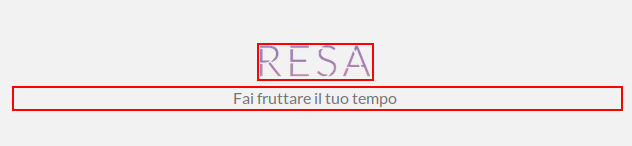
\includegraphics[width=.8\columnwidth]{images/dashboardLink.png}
		\caption{Link al sottomodulo \resa{} (le parti cliccabili sono circondate dai rettangoli rossi)}
	\end{figure}
	
	\item Sul \textit{menù laterale} la pagina corrente viene evidenziata colorando diversamente
	l'area circostante il nome, questo potrebbe dare la falsa impressione che tutta quell'area
	sia cliccabile quando in realtà soltanto il testo lo è, si tratta di un falso indizio che
	potrebbe portare ad errori da parte delle/degli utenti. Buona idea sarebbe rendere cliccabile
	tutta l'area.
	
	\begin{figure}[H]\label{imgLeftNav}
	\centering
	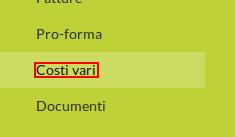
\includegraphics[width=.4\columnwidth]{images/areacliccabile.png}
	\caption{Esempio di colorazione per evidenziare la pagina corrente (l'area cliccabile è circondata dal rettangolo rosso)}
	\end{figure}
		
	\item Su \textit{\resa{}}, per chiudere la finestra del timer delle attività e necessario cliccare
	all'interno di essa. Questo presenta due problemi, il primo è che non è intuitivo dover
	cliccare su di un elemento per chiuderlo (normalmente bisogna cliccare all'esterno e questo
	è ad esempio il comportamento della menù laterale di navigazione), il secondo è che è
	possibile che un/a utente sbagli ad esempio nel cliccare il tasto "play", chiudendo la
	finestra.
	\end{itemize}
\item \textbf{Colorazione e contrasti}: tutti gli elementi di una pagina dovrebbero
essere facilmente visibili agli utenti, anche in caso di problemi di vista, ecc.
	\begin{itemize}
	\item I \textit{titoli} delle pagine, su Firefox, si vedono molto chiari sullo sfondo,
	questo potrebbe causare problemi di visualizzazione.
	
	\begin{figure}[H]\label{imgContrasti}
	\centering
	
\includegraphics[width=.4\columnwidth]{images/contrasti.png}
	\caption{Esempio di contrasto tra il titolo di una pagina e lo sfondo}
	\end{figure}
	
	\end{itemize}
\item \textbf{Coerenza e prevedibilità delle azioni degli/delle utenti}: una azione di un/a
utente dovrebbe sempre dare lo stesso risultato. Le sorprese non sono gradite e un sito
dal comportamento "imprevedibile" genera frustrazione.
	\begin{itemize}
	\item Il \textit{logo} posto in alto a sinistra sulle diverse pagine del sito dà al click
	risultati diversi in situazioni diverse: se il menù laterale è aperto, lo chiude, se invece
	il menù è chiuso, porta alla pagina di Scrivania. Questo è dovuto al fatto che
	\textit{un qualsiasi} click al di fuori del menù ne causa la chiusura, e questo evento ha
	priorità rispetto a quello di redirect sulla pagina di Scrivania. Questo però è un dettaglio
	tecnico ignoto alle/agli utenti i quali potrebbero non gradire questa diversità di esiti.
	\end{itemize}
\item \textbf{Tracciabilità del proprio percorso}: è importante per un/a utente poter
ripercorrere i propri passi all'interno di un sito web e in generale poter capire in ogni
momento a colpo d'occhio la propria posizione nella gerarchia del sito, per questo sono
utili degli strumenti come ad esempio i \textit{breadcrumb}
	\begin{itemize}
	\item Nelle pagine di secondo di livello del sito (come ad esempio la pagina di
	\textit{creazione di una nuova fattura}) non sono presenti dei breadcrumb. Per tornare alla
	pagina precedente sarebbe necessario utilizzare il tasto \textit{back} del browser oppure
	aprire il menù e riselezionarla.
	\end{itemize}
\item \textbf{Evidenziare le funzionalità}: una qualsiasi funzionalità deve sempre essere
messa chiaramente in evidenza, se un'area di testo è editabile si deve poter capire a colpo
d'occhio, se una zona è cliccabile anche, ecc.
	\begin{itemize}
	\item Su \textit{\resa{}}, nel box di creazione rapida delle attività non è immediatamente
	evidente che i valori di minuti e ore del tempo stimato siano editabili come una normale
	textbox. Gli altri campi di testo editabili sono circondati da un bordo che li identifica
	convenzionalmente come tali.
	
	\begin{figure}[H]\label{imgCreazioneAttivita}
	\centering
	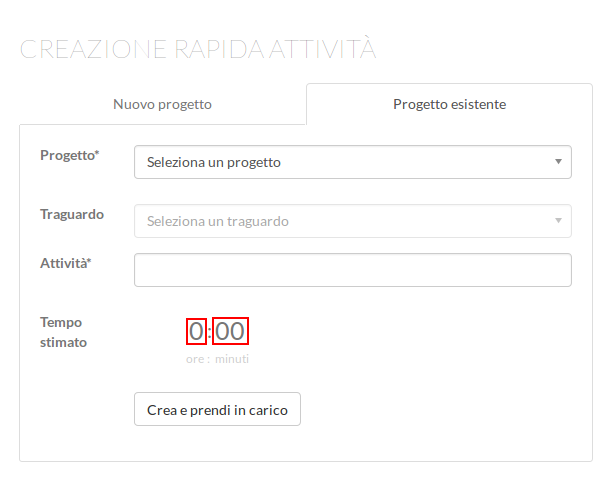
\includegraphics[width=.8\columnwidth]{images/creazioneAttivita.png}
	\caption{Box di creazione rapida delle attività, le parti circondate dai rettangoli rossi sono editabili come normali text box}
	\end{figure}
		
	\end{itemize}
\end{itemize}

\subsection{Aspetti positivi}
L'applicazione presenta alcuni aspetti positivi che contribuiscono a migliorare l'esperienza
delle/degli utenti.

\begin{itemize}
\item \textbf{Aiuto contestuale}: per un'applicazione web contemporanea non ha molto senso
fornire un manuale d'uso "classico". Gli/Le utenti sono ormai abituati/e ad esplorare da
subito le diverse funzionalità, imparando mano a mano che scoprono il prodotto.
\fiscoloWeb{} offre in diverse occasioni un aiuto contestuale, ovvero delle informazioni
semplici e rapide su come portare a termine un obiettivo, date nel contesto giusto, ovvero
quando l'utente sta effettivamente perseguendo quell'obiettivo. Oltre a questo vengono
fornite anche una guida approfondita e completa come riferimento e una funzionalità di help
che apre un box esplicativo per ogni pagina.

\begin{figure}[H]\label{imgAiutoContestuale}
\centering
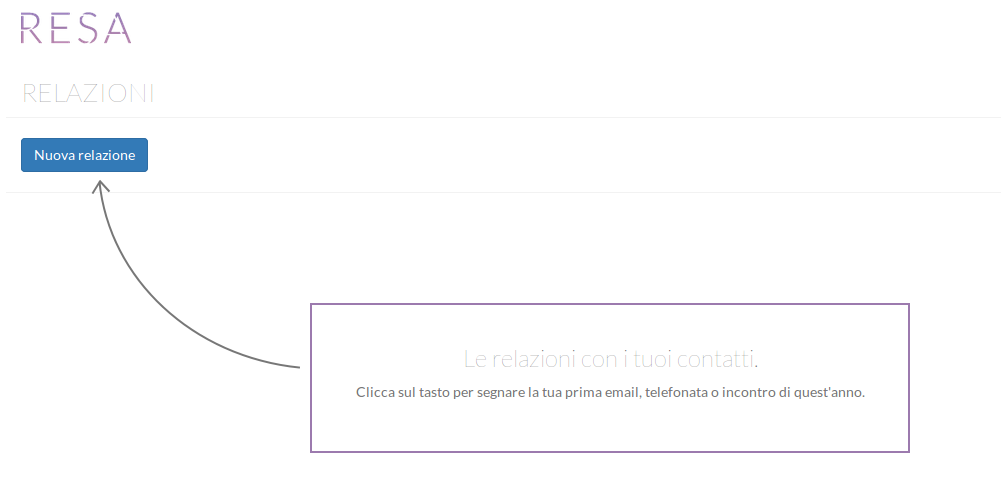
\includegraphics[width=1\columnwidth]{images/aiutoContestuale.png}
\caption{Esempio di aiuto contestuale su \resa}
\end{figure}

\item \textbf{Consistenza della presentazione grafica}: i due sottomoduli sono ben divisi
dagli schemi di colorazione e dai loghi posti in alto a sinistra delle pagine, questo permette
di capire a colpo d'occhio in che macro-area dell'applicazione ci si trova.
\end{itemize}
\section{Glossario}

\begin{itemize}
\item \textbf{Attività}: in \fiscolo{} un'Attività è sempre parte di un \gloss{Progetto},
ha un tempo preventivato e un tempo consuntivato (inserito manualmente o calcolato tramite
il timer offerto dall'applicazione). Può essere assegnata a degli/delle utenti o presa
in carico dagli stessi/dalle stesse.

\item \textbf{Contatto}: in \fiscolo{} un Contatto rappresenta semplicemente un referente
per una o più aziende.

\item \textbf{Costo}: in \fiscolo{} un Costo è definito da una data, un importo, una
descrizione ed una categoria, tali categorie sono definite dagli utenti e possono aumentare
in modo arbitrario.

\item \textbf{Data binding}: si tratta di una connessione tra l'interfaccia utente ed
elementi della logica di business (i.e. i dati) di un'applicazione.

\item \textbf{ISO}: acronimo per \textit{Internation Organization for Standardization}.

\item \textbf{JSON}: acronimo per \textit{JavaScript Object Notation}, si tratta di un formato
di scambio dati fra applicazioni client-server.

\item \textbf{Markup}: si tratta di linguaggi standardizzati che permettono di scrivere un
testo definendone allo stesso tempo alcune proprietà strutturali e semantiche. In questa
relazione ci si riferisce al linguaggio HTML.

\item \textbf{MVC}: acronimo per \textit{Model View Controller}

\item \textbf{MVVM}: acronimo per \textit{Model View View Model}

\item \textbf{MVW}: acronimo per \textit{Model View Wathever}

\item \textbf{NOOP}: si tratta di un comando la cui invocazione non ha effetti di alcun
tipo

\item \textbf{Progetto}: in \fiscolo{} un Progetto è visto come un insieme di \gloss{attività}
che possono essere relazionate a dei \gloss{traguardi}.

\item \textbf{Promemoria}: in \fiscolo{} un Promemoria consiste di un testo (di lunghezza
qualsiasi) al quale è associata la data di creazione. Può essere attivo o concluso.

\item \textbf{Relazione}: in \fiscolo{} una Relazione è definita da una data, una tipologia
(email, incontro o telefonata), uno o più \gloss{contatti}, una descrizione ed un eventuale
indirizzo.

\item \textbf{REST}: acronimo per \textit{REpresentational State Transfer}, si riferisce a
interfacce che permettono di trasmettere dati su HTTP senza necessità di sessioni o di
mantenimento di stato.

\item \textbf{Tap}: modalità di interazione mobile che consiste nella rapida pressione
di un'area di schermo con il dito.

\item \textbf{Touch ripple}: nome dato a una reazione visiva associata al tocco di un
particolare componente, l'effetto è quello di un'onda che si propaga come accade sulle
superfici liquide

\item \textbf{Traguardo}: si tratta in sostanza di quelle che nel gergo dell'Ingegneria del
Software vengono chiamate \textit{milestone}. Sono scadenze di una certa importanza come
rilasci, revisioni di avanzamento, ecc.

\item \textbf{Usabilità}: viene definita dall'\gloss{ISO} come \textit{l'efficacia, l'efficienza
e la soddisfazione con le quali determinati utenti raggiungono determinati obiettivi in
determinati contesti}. Uno studio dell'usabilità di un'applicazione o di un sito web ne valuta
dunque l'intuitività e la possibilità di un utilizzo sereno da parte degli/delle utenti.
\end{itemize}
\section{Sitografia}

\renewcommand{\section}[2]{}
\begin{thebibliography}{9}

\bibitem{lukew} Articoli di Luke Wroblewski - \texttt{http://www.lukew.com/ff/}
\bibitem{luke-pass} Sulla mascheratura delle password - \texttt{http://www.lukew.com/ff/entry.asp?1941}
\bibitem{pass-test} Test effettuato sulla mascheratura delle password - \texttt{ http://passwordmasking.com/}
\bibitem{luke-dropdown} Sui menù a tendina - \texttt{http://www.lukew.com/ff/entry.asp?1950}

\end{thebibliography}

\end{document}